% Report for MATH6641 Project
% Copyright (C) 2018 Andrew Johnson, GTRC
% This program is free software: you can redistribute it and/or modify
% it under the terms of the GNU General Public License as published by
% the Free Software Foundation, either version 3 of the License, or
% (at your option) any later version.
% 
% This program is distributed in the hope that it will be useful,
% but WITHOUT ANY WARRANTY; without even the implied warranty of
% MERCHANTABILITY or FITNESS FOR A PARTICULAR PURPOSE.  See the
% GNU General Public License for more details.
% 
% You should have received a copy of the GNU General Public License
% along with this program.  If not, see <http://www.gnu.org/licenses/>.
\documentclass{article}
\usepackage{amsmath}
\usepackage{booktabs}
\usepackage{tikz}
\newcommand{\mfesv}{\mathcal{V}_h}
\newcommand{\tauh}{\mathcal{T}_h}
\newcommand{\pdiff}[2]{\frac{\partial#1}{\partial#2}}
\newcommand{\ddx}[1]{\pdiff{#1}{x}}
\newcommand{\ddt}[1]{\pdiff{#1}{t}}
\newcommand{\dpmdx}{\ddx{\psi_m}}
\newcommand{\dpmdt}{\ddt{\psi_m}}
\newcommand{\fisTrms}{\chi\nu\sigma_f}
\newcommand{\tfor}{\text{ for }}
\newcommand{\tfes}{finite-element space }
\newcommand{\forEtaInV}{,\,\forall\eta\in\mfesv}
\newcommand{\sumTaus}{\sum_{\tauinT}}
\newcommand{\tfem}{finite-element method }
\newcommand{\tauinT}{\tau\in\tauh}
\newcommand{\fepsim}{\tilde{\psi}_m}
\newcommand{\fepsimj}{\tilde{\psi}_{m,j}}
\newcommand{\invv}{\frac{1}{v}}
\newcommand{\innerProd}[2]{\left(#1,#2\right)}
\newcommand{\tauInt}[2]{\innerProd{#1}{#2}_\tau}
\newcommand{\ajl}{\alpha_{j,l}}
\newcommand{\inTau}[1]{\left.#1\right\vert_{\tau}}
\title{$FeS_NT$ - A Finite Element Neutron Transport Solver}
\author{Andrew Johnson}
\usepackage[left=1in,right=1in,top=0.75in,bottom=1in]{geometry}
\usepackage{cleveref}

\begin{document}

\maketitle

\section{Introduction}
The goal of this work is to introduce and explain the code written for the MATH6641 project.
The time-dependent one-dimensional neutron transport equation was solved using the discrete 
ordinates formulation \textbf{cite} using discontinuous-Galerkin in space, and
explicit Euler for time.
The project was written in Python and works best with 3.5\footnote{not tested on other versions}
and is included with this report in \texttt{fesnt.py}.
This report, and the code included, are covered with the GNU Public License, found in \texttt{LICENSE}.

\subsection{Problem Statement}
The discrete-ordinates formulation of the neutron transport equation chooses to solve for the angular
neutron flux, $\psi(x, \mu, t)$ along a discrete set of $N$ angles $\vec{\mu}$. A quadrature set of 
weights and angles is chosen to satisfy some physical constraints, briefly summarized here:
\begin{subequations} \label{eq:quadRules}
    \begin{equation}
        \mu_m = -\mu_{N-m+1}
    \end{equation}
    \begin{equation}
        w_m = w_{N-m+1}
    \end{equation}
    \begin{equation}
        \sum_m w_m = 2
    \end{equation}
    \begin{equation}
        \int_{-1}^1f(x, \mu)d\mu\approx\sum_mw_m f(x, \mu_m)
    \end{equation}
\end{subequations}

The weights and angles are, for this work, chosen from a Guass-Legendre polynomial set.
%TODO: verify and cite
Select sets of weights and angles are listed in \cref{sec:qsets}

This project seeks to solve the following initial-boundary value problem:
\begin{equation} \label{eq:ibvpNTE}
    \frac{1}{\nu}\dpmdt+\mu_m\dpmdx+\sigma_t(x)\psi(x, t) = 
    \sigma_S(x)\phi(x, t), \tfor a<x<b,t>0, \mu_m\in\vec{\mu}
\end{equation}
where
\begin{equation}
    \phi(x, t) = \sum_mw_m\psi_m(x, t)
\end{equation}
and $\sigma_S(x) =\frac{1}{2}\left(\sigma_s(x) + \fisTrms(x)\right)$.

\Cref{eq:ibvpNTE} is subject to initial and boundary conditions
\begin{subequations}
    \begin{equation}
        \psi_m(x, 0) = \psi_{m,0}(x), \tfor a<x<b, \mu_m\in\vec{\mu}
    \end{equation}
    \begin{equation}
        \psi_m(a, t) = \Gamma_a(\mu_m, t)\tfor \mu_m>0,t>0
    \end{equation}
    \begin{equation}
        \psi_m(b, t) = \Gamma_b(\mu_m, t)\tfor\mu_m<0, t>0
    \end{equation}
\end{subequations}

The report is laid out as follows. \Cref{sec:derive} derives the numerical scheme implemented
for this project. \Cref{sec:implement} gives some insight into the actual implementation
and usage needed to reproduce the results. \Cref{sec:results} presents results from
three test cases of increasing difficulty.

\section{Derivation of the Method} \label{sec:derive}
The author set out to apply a finite-element scheme for the spatial domain, with an implicit Euler
scheme in time. This section shall detail the mathematical foundation for the project, and present the
numeric scheme that was ultimately implemented for this work.

\subsection{Notation}
Following the work of Reed and Hill \cite{wReed1973}, 
the author set out to apply a Discontinuous-Galerkin (DG) method for the spatial domain.
This required subdividing the domain $a<x<b$ into non-overlapping elements $\tau$.
The \tfes $\mfesv$ was chosen to be piece-wise quadratic polynomials that are continuous 
within a single element.

\subsubsection{Finite-Element Spaces}
The following \tfes was used for the trial functions that approximated $\psi(x,\mu, t)$ within an
element $\tau$. Let $\mfesv$ be the space
\begin{equation}
    \label{eq:vhspace}
    \begin{split}
        \mfesv = \lbrace \fepsim\vert & \fepsim \text{ is piece-wise quadratic}, \\
            & \fepsim(a, \mu, t) = 
                \begin{cases}
                    \Gamma_a(\mu, t), \text{ if } \mu>0\\
                    0,\text{ otherwise}
                \end{cases}, \\
            & \fepsim(b, \mu, t) = 0 \rbrace
    \end{split}
\end{equation}

For this work, the test functions used to create the \tfem were of the piece-wise quadratic within each
mesh and taken to be
\begin{equation}
    \label{eq:testfuncs}
    \eta_i(x) = x^i
\end{equation}
which, for $i\leq2$, is contained within $\mfesv$.


\subsubsection{Quadratic Flux}
Within each element $\tau$, the flux was represented as a quadratic function using the element boundaries and 
midpoint of the element.
Specifically, the angular flux was represented using Lagrange interpolating polynomials, as
\begin{equation}
    \label{eq:fluxPoly}
    \fepsim(x) = \sum_{j=0}^2\fepsimj\sum_{l=0}^2\ajl x^l
    = \sum_{j=0}^2\fepsimj\prod_{l=0,l\neq j}^2\frac{x-x_l}{x_j-x_l}
\end{equation}
This way, given three internal points of element $\tau$, the Lagrange coefficients
$\ajl$ could be determined, meaning that amplitudes $\fepsimj$ remained to
be solved.
Using this notation, the spatial derivative of the flux is expressed as
\begin{equation}
    \label{eq:fluxDeriv}
    \pdiff{\fepsim}{x} = \sum_{j=0}^2\fepsimj\sum_{l=1}^2l\ajl x^{l-1}
\end{equation}
The benefit of using Lagrange polynomials is that, at a specific lattice site $x_l$, the 
angular flux evaluates to the specific polynomial amplitude, i.e.
\begin{equation}
    \tilde{\psi}_m(x_j) =\fepsimj 
\end{equation}

Using a quadratic representation of the flux within an element allows the use of Simpson's
integration without introducing additional error, as such a method is exact for polynomials
of order 2 or less.
According to Simpson's rule, the spatial integral of a function can be expressed as
\begin{equation}
    \label{eq:simpsInt}
    \int_a^bf(x)dx \approx \frac{b-a}{2}\left(f(a) + 4f\left(\frac{b-a}{2}\right) + f(b)\right)
\end{equation}

\subsubsection{Upwind/Downwind Elements}
The scheme implemented iterates through all angles in the quadrature set, and marches through
elements in a manner akin to following the wind-direction. When $mu$ is less than zero, this 
translates to moving left along the $x$ axis, and the first mesh is taken to be the mesh
with an edge at $x=b$. 
Such a scheme requires distinctions to be made between upwind and downwind sides, as will be utilized
heavily in later sections. \Cref{fig:upwDnw} describes the upwind side of the edges of element $\tau$
as $-$ sides, and downwind sides as $+$.

\begin{figure}
    \centering
    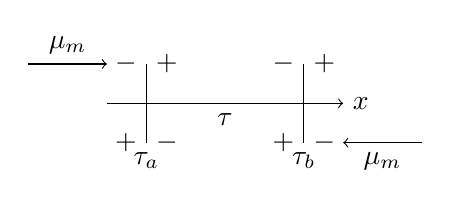
\begin{tikzpicture}
        % tikz picture for displaying the +/- sides of each element
% given an angle

\draw[->] (-0.5, 0) -- (2.5, 0) 
    node[pos=0.5, below]{$\tau$} 
    node[pos=1, right]{$x$};
\draw (0, -0.5) -- (0, 0.5) 
    node[pos=0, left]{$+$} 
    node[pos=0, right]{$-$} 
    node[pos=0, below]{$\tau_a$}
    node[pos=1, left]{$-$} 
    node[pos=1, right]{$+$};
\draw (2, -0.5) -- (2, 0.5) 
    node[pos=0, left]{$+$} 
    node[pos=0, right]{$-$}
    node[pos=0, below]{$\tau_b$}
    node[pos=1, left]{$-$} 
    node[pos=1, right]{$+$};
\draw[<-] (-0.5, 0.5) -- (-1.5, 0.5) 
    node[pos=0.5, above]{$\mu_m$};
\draw[->] (3.5, -0.5) -- (2.5, -0.5) 
    node[pos=0.5, below]{$\mu_m$};

    \end{tikzpicture}
    \caption{Notation used to denote upwind and downwind elements given flux angle $\mu$}
    \label{fig:upwDnw}
\end{figure}

Using this distinction, the jump of a function across an element edge is defined with
\begin{subequations}
    \begin{equation}
        V^+ = \lim_{s\rightarrow 0^+}V(x+s\mu)
    \end{equation}
    \begin{equation}
        V^- = \lim_{s\rightarrow 0^-}V(x+s\mu)
    \end{equation}
    \begin{equation}
        \label{eq:jumpDef}
        \left[V(x)\right] = V^+-V^-
    \end{equation}
\end{subequations}

\subsection{Finite-Element Method}
Given these definitions, the process for deriving the \tfem can begin. 
To start, multiply \cref{eq:ibvpNTE} by a test function $\eta_i\in\mfesv$ and integrating over
the spatial domain $\Omega=[a,b]$.
If the spatial discretization $\mathcal{T}_h$ does not cross material boundaries, then cross sections $\sigma_S$
are constant within an element.
The finite element will seek to approximate
\begin{equation}
    \label{eq:derive0}
    \sumTaus\left[
        \invv\tauInt{\dpmdt}{\eta}
        +\mu_m\tauInt{\dpmdx}{\eta}
        +\sigma_{t,\tau}\tauInt{\psi_m}{\eta}
    \right]
    = \sumTaus\sigma_S\tauInt{\phi}{\eta}
    \forEtaInV
\end{equation}

By integrating the spatial derivative term by parts, the derivative can be shifted off
the true function $\psi$\footnote{assumed to be sufficiently smooth}.
\begin{equation}
    \tauInt{\dpmdt}{\eta} = \left.\left[\overset{*}{\psi_m}\inTau{\eta}\right]\right\vert_{\tau_a}^{\tau_b}
        -\tauInt{\psi_m}{\ddx{\inTau{\eta}}}
\end{equation}

Here, caution must be taken to ensure that the test function is evaluated \textit{inside} the
element $\tau$.
Since $\psi_m$ is sufficiently smooth, we can take the upwind information $\overset{*}{\psi_m}=\fepsim^-$,
but choosing $\inTau{\eta}$ to always be inside the element.
Another integration by parts, replacing $\psi_m\rightarrow\fepsim$ as the derivative has been removed
\begin{equation}
    \label{eq:derive1}
    \tauInt{\fepsim}{\ddx{\inTau{\eta}}}=\left.\left[
        \overset{**}\psi_m\inTau{\eta}
    \right]\right|_{\tau_a}^{\tau_b}
    -\tauInt{\inTau{\ddx{\fepsim}}}{\eta}
\end{equation}

Here, $\overset{**}{\psi_m}$ must be taken inside $\tau$, yielding
\begin{equation}
    \label{eq:derive2}
    \tauInt{\dpmdx}{\eta}\Rightarrow
        \tauInt{\inTau{\ddx{\fepsim}}}{\eta}
        + \left.\left[\left(\overset{*}\psi_m-\overset{**}{\psi_m}\right)\inTau{\eta}\right]
        \right\vert_{\tau_a}^{\tau_b}
\end{equation}

For positive of negative values of $\mu$, different terms in \cref{eq:derive2} will cancel.
For $\mu>0$,

\section{Implementation} \label{sec:implement}

\subsection{Using \texttt{fesnt.py}} \label{sec:usage}

\section{Results} \label{sec:results}

\subsection{Case 1: Pure-Absorber} \label{sec:pa}

\subsection{Case 2: Non-fissile} \label{sec:nonFissile}

\subsection{Case 3: Fissile Problem} \label{sec:fissile}

\section{Conclusion} 

\bibliography{./refs.bib}
\bibliographystyle{IEEEtran}

\section{Appendix}

\subsection{Quadrature Sets} \label{sec:qsets}
The following tables contain the quadrature sets that were used in this work.
For each set, only half of the values are presented, as symmetry rules from \cref{eq:quadRules}
can be used to construct the full set.
%TODO: Cite L&M
%TODO:W: Two columns

\begin{table}[h!]
    \caption{S-2 Weights and Angles}
    \label{tb:s2quad}
    \centering
    \begin{tabular}{cc}
        \toprule
        $\mu_m$ & $w_m$ \\
        \midrule
        0.5773502691 & 1.0 \\
        \bottomrule
    \end{tabular}
\end{table}

\begin{table}[h!]
    \caption{S-4 Weights and Angles}
    \label{tb:s4quad}
    \centering
    \begin{tabular}{cc}
        \toprule
        $\mu_m$ & $w_m$ \\
        \midrule
        0.3399810435 & 0.6521451549 \\
        0.8611363115 & 0.3478548451 \\
        \bottomrule
    \end{tabular}
\end{table}

\begin{table}[h!]
    \caption{S-8 Weights and Angles}
    \label{tb:s8quad}
    \centering
    \begin{tabular}{cc}
        \toprule
        $\mu_m$ & $w_m$ \\
        \midrule
        0.1834346424 & 0.3626837834 \\
        0.5255324099 & 0.3137066459 \\
        0.7966664774 & 0.2223810344 \\
        0.9602898564 & 0.1012285363 \\
        \bottomrule
    \end{tabular}
\end{table}


\end{document}

